       \documentclass[journal, a4paper]{IEEEtran}

% some very useful LaTeX packages include:

%\usepackage{cite}      % Written by Donald Arseneau
                        % V1.6 and later of IEEEtran pre-defines the format
                        % of the cite.sty package \cite{} output to follow
                        % that of IEEE. Loading the cite package will
                        % result in citation numbers being automatically
                        % sorted and properly "ranged". i.e.,
                        % [1], [9], [2], [7], [5], [6]
                        % (without using cite.sty)
                        % will become:
                        % [1], [2], [5]--[7], [9] (using cite.sty)
                        % cite.sty's \cite will automatically add leading
                        % space, if needed. Use cite.sty's noadjust option
                        % (cite.sty V3.8 and later) if you want to turn this
                        % off. cite.sty is already installed on most LaTeX
                        % systems. The latest version can be obtained at:
                        % http://www.ctan.org/tex-archive/macros/latex/contrib/supported/cite/
 \usepackage{algorithm}
\usepackage[noend]{algpseudocode}
\makeatletter
\def\BState{\State\hskip-\ALG@thistlm}
\makeatother
\usepackage{amssymb}
\usepackage{graphicx}
\graphicspath{ {images/} }   % Written by David Carlisle and Sebastian Rahtz
                        % Required if you want graphics, photos, etc.
                        % graphicx.sty is already installed on most LaTeX
                        % systems. The latest version and documentation can
                        % be obtained at:
                        % http://www.ctan.org/tex-archive/macros/latex/required/graphics/
                        % Another good source of documentation is "Using
                        % Imported Graphics in LaTeX2e" by Keith Reckdahl
                        % which can be found as esplatex.ps and epslatex.pdf
                        % at: http://www.ctan.org/tex-archive/info/

%\usepackage{psfrag}    % Written by Craig Barratt, Michael C. Grant,
                        % and David Carlisle
                        % This package allows you to substitute LaTeX
                        % commands for text in imported EPS graphic files.
                        % In this way, LaTeX symbols can be placed into
                        % graphics that have been generated by other
                        % applications. You must use latex->dvips->ps2pdf
                        % workflow (not direct pdf output from pdflatex) if
                        % you wish to use this capability because it works
                        % via some PostScript tricks. Alternatively, the
                        % graphics could be processed as separate files via
                        % psfrag and dvips, then converted to PDF for
                        % inclusion in the main file which uses pdflatex.
                        % Docs are in "The PSfrag System" by Michael C. Grant
                        % and David Carlisle. There is also some information
                        % about using psfrag in "Using Imported Graphics in
                        % LaTeX2e" by Keith Reckdahl which documents the
                        % graphicx package (see above). The psfrag package
                        % and documentation can be obtained at:
                        % http://www.ctan.org/tex-archive/macros/latex/contrib/supported/psfrag/

%\usepackage{subfigure} % Written by Steven Douglas Cochran
                        % This package makes it easy to put subfigures
                        % in your figures. i.e., "figure 1a and 1b"
                        % Docs are in "Using Imported Graphics in LaTeX2e"
                        % by Keith Reckdahl which also documents the graphicx
                        % package (see above). subfigure.sty is already
                        % installed on most LaTeX systems. The latest version
                        % and documentation can be obtained at:
                        % http://www.ctan.org/tex-archive/macros/latex/contrib/supported/subfigure/

\usepackage{url}        % Written by Donald Arseneau
                        % Provides better support for handling and breaking
                        % URLs. url.sty is already installed on most LaTeX
                        % systems. The latest version can be obtained at:
                        % http://www.ctan.org/tex-archive/macros/latex/contrib/other/misc/
                        % Read the url.sty source comments for usage information.

%\usepackage{stfloats}  % Written by Sigitas Tolusis
                        % Gives LaTeX2e the ability to do double column
                        % floats at the bottom of the page as well as the top.
                        % (e.g., "\begin{figure*}[!b]" is not normally
                        % possible in LaTeX2e). This is an invasive package
                        % which rewrites many portions of the LaTeX2e output
                        % routines. It may not work with other packages that
                        % modify the LaTeX2e output routine and/or with other
                        % versions of LaTeX. The latest version and
                        % documentation can be obtained at:
                        % http://www.ctan.org/tex-archive/macros/latex/contrib/supported/sttools/
                        % Documentation is contained in the stfloats.sty
                        % comments as well as in the presfull.pdf file.
                        % Do not use the stfloats baselinefloat ability as
                        % IEEE does not allow \baselineskip to stretch.
                        % Authors submitting work to the IEEE should note
                        % that IEEE rarely uses double column equations and
                        % that authors should try to avoid such use.
                        % Do not be tempted to use the cuted.sty or
                        % midfloat.sty package (by the same author) as IEEE
                        % does not format its papers in such ways.

\usepackage{amsmath}    % From the American Mathematical Society
                        % A popular package that provides many helpful commands
                        % for dealing with mathematics. Note that the AMSmath
                        % package sets \interdisplaylinepenalty to 10000 thus
                        % preventing page breaks from occurring within multiline
                        % equations. Use:
%\interdisplaylinepenalty=2500
                        % after loading amsmath to restore such page breaks
                        % as IEEEtran.cls normally does. amsmath.sty is already
                        % installed on most LaTeX systems. The latest version
                        % and documentation can be obtained at:
                        % http://www.ctan.org/tex-archive/macros/latex/required/amslatex/math/



% Other popular packages for formatting tables and equations include:

%\usepackage{array}
% Frank Mittelbach's and David Carlisle's array.sty which improves the
% LaTeX2e array and tabular environments to provide better appearances and
% additional user controls. array.sty is already installed on most systems.
% The latest version and documentation can be obtained at:
% http://www.ctan.org/tex-archive/macros/latex/required/tools/

% V1.6 of IEEEtran contains the IEEEeqnarray family of commands that can
% be used to generate multiline equations as well as matrices, tables, etc.

% Also of notable interest:
% Scott Pakin's eqparbox package for creating (automatically sized) equal
% width boxes. Available:
% http://www.ctan.org/tex-archive/macros/latex/contrib/supported/eqparbox/

% *** Do not adjust lengths that control margins, column widths, etc. ***
% *** Do not use packages that alter fonts (such as pslatex).         ***
% There should be no need to do such things with IEEEtran.cls V1.6 and later.


% Your document starts here!
\begin{document}

% Define document title and author
    \title{Analyzing the Impact of Move-In Week on the Greater Boston Area}
    \author{Brooke Mullen, Claire Russack, Dharmesh Tarapore, Vincent Wahl
    \\bemullen@bu.edu, crussack@bu.edu, dharmesh@bu.edu, vinwah@bu.edu
    }
    \markboth{Boston University: CS 591 L1}{}
    \maketitle

% Write abstract here
\begin{abstract}
    Move in week is universally chaotic and a generally unpleasant experience for both, college students and local residents \cite{painfulmovein}. Despite universities' meticulous attempts to mitigate trouble, the logistical concerns presented by the sudden influx of over 30,000 students are inevitable. In this project, we attempt to identify specific factors affecting residents' quality of life (as a result of move-in week) and study ways to improve it.   
\end{abstract}

% Each section begins with a \section{title} command
\section{Introduction}
    % \PARstart{}{} creates a tall first letter for this first paragraph
    \IEEEPARstart{}Over 50,000 new and returning students move in to dormitories and apartments in the city of Boston each year \cite{moveinstats}. Known colloquially as "move-in week", this 7-day period between late August and early September wreaks considerable havoc over residents' lives. Traffic delays, overcrowded public transport, inadequate parking spaces, and the infamous \textit{"Storrowed"} trucks \cite{storrowed} are among some of the difficulties that irk both, students and locals.
\\Due to the nature of an academic calendar for most universities, the lease cycle tends to be September 1st. This rapid movement in a dense area affects the overall quality of life in the city, often for the worse. In this project, we attempt to isolate the true impact of college students moving in on the locals' lives and ways to mitigate the worst effects of move-in week.
\\Mensurability notwithstanding, conventional proxies\footnote{The GDP (Gross Domestic Product) is often used as an approximate measure of quality of life, in conjunction with other metrics such as the HDI (Human Development Index) and Gini Coefficient.} for quality of life disregard (among other things) societal happiness: a critical adjunct to traditional economic metrics \cite{happytext}. 
To remedy this, we propose an approach that utilizes open data sourced from Boston City's \textit{Analyze Boston} data portal \cite{bosdatalink} and posts made on the microblogging platform, Twitter \cite{twitterlink}. In particular, we use the \textit{CityScore}, \textit{311 Service Requests}, and \textit{Boston Fire Incident Reporting} datasets to identify the demand for specific city resources across multiple time periods as a function of user satisfaction.
\\The rest of this paper is organized as follows: in section II, we document related research that inspired this project. In section III, we describe each of the 4 chosen datasets in greater detail to focus on their merits, potential limitations, and the methods we used to discern their relative importance in estimating the city's quality of life. Section III also outlines our results and examines their implications. Section IV concludes the report with an outlook on future research.
%To quantify the quality of the city on a given day, we used the Analyze Boston's City Score dataset. The Boston City Score is an initiative created to monitor the overall health of the city on a daily basis. It is calculated by aggregating various metrics, both additive and negative, into a single score. This dataset is one that was central to our project and was used as a significant way of determining metrics had on the quality of life.
%A solution that the city poses is temporary parking and traffic restrictions in areas that usually surround areas with a high density of student movers. Due to minimal options for transportation and the high movement, renters do not have space or resources to deal with their trash and furniture, leaving them to dispose of it in their surroundings. It is not surprising to find refrigerators, mattresses, and desks littered along the sides of the streets during this time. Analyze Boston's 311 Service Requests records these violations and their locations. With the understanding that the number of violations affects the quality of life on a given day in Boston, one of our aims became to find a way to serve requests in the most timely way. To make this solution concrete but also efficient, our team worked to display the minimum number of dispatchers required to respond to service requests within 30 seconds of each inquiry. 
%Another metric that affects the quality of life in Boston is fire incidents in the city. The dataset, ‘Fire Incident Reporting’, also comes from Analyze Boston. The data set consists of incident details and location. It is non-trivial that a residential or commercial fire will negatively affect the quality of life so our question became finding the mean point of where incidents occur. 
%In the City Score dataset, one of the features quantifies the amount of public library users on a given day. This metric is one that is additive to the city score. While students could potentially be detrimental to the quality of Boston’s life, it was possible that they could also be boosting it with increased library attendance. Two different datasets were created from City Score based on the library attendance metric. The first consisted of attendance when university was in session and the second was when it was not in session. 

% Related Work
\section{Related Work}
    Jim Haddadin explored the relationship between move-in week and garbage disposal concerns in \cite{trashcity}. Noting a sharp rise in the number of code violations around university residences during move-in week, Haddadin highlights some unforeseen consequences of improper trash disposal. In \cite{happytext}, Dodds et al address the subjectivity and vagueness inherent to estimating happiness among people by mining over 46 billion tweets to uncover temporal variations in happiness and information levels over timescales ranging from hours to years.Their remote-sensing 'hedonometer' algorithm generated a rich source of information about short-term, experiential happiness in a population and its causes. We use a similar, albeit slightly modified approach to understand residents' moods during move-in week.

\section{Approach and Results}
Our desire to allay the worst aspects of move-in week presupposes the existence of a correlation between students moving in and a perceptible change in the quality of residents' lives. This requires: 
\\ \null \quad\quad i. The identification of metrics that can effectively approximate quality of life and
\\\null\quad\quad ii. Predictive analyses that capture and justify the impact of altering select attributes of move-in week\footnote{Note that this does \textbf{not} insinuate the existence of a causal relationship between university students moving in and residents' quality of life: it merely seeks to leverage potential correlations between the two.}.
\\Similar to the approaches charted in \cite{happytext} and \cite{trashcity}, we begin first by selecting datasets that might evince the impact of students moving in. Boston City's Open Data Initiative, \textit{Analyze Boston} portal provides a vast repository of highly granular information about the city's functioning. In particular, the \textit{311 Service Requests}, \textit{CityScores}, and \textit{Fire Incident Reporting} datasets are of particular interest and we expound their significance below \cite{bosdatalink}. For quality of life, we rely on the seminal research conducted by Mitchell et al in \cite{happytexttwitter} and use geotagged Twitter posts within 50 kilometers of Boston city to gauge happiness. Limitations stemming from a lack of representativeness and potential bias in dataset selection are explored further in section IV.

\subsection{311 Service Requests} 
Analyze Boston��s 311 Service Request provides records of non-emergency city
violations, such as improper trash disposal and illegal parking complaints, along
with the date and time of the incident being reported and the location of these in
incidents. With the understanding that the number of violations affects the quality
of life on a given day in Boston, one of our aims became to find both the sum of
number of incidents for a given period as well as the minimum number of service
request dispatchers required to simply respond to the incoming requests. The
minimum number of dispatchers is determined by the minimum number people
required to respond to incoming inquiries such that no incoming inquiry is queued
or rejected.

Since we are interested in the quality of life of residents and students, we chose to
filter the incoming requests such that all requests that were clearly related to
businesses were removed. This way, the requests would represent distress to
residents as a result of other residents. Given that the 311 Service Request data only
provides the starting time of such inquiries, we chose to assume that every inquiry
has a length of 3 minutes.

First all service requests in the period $2016/02/01$ to $2018/03/30$ were retrieved
from Analyze Boston at the $4^{th}$ of April $2018$. The retrieved data, was then filtered to
only include relevant inquiries, such as: Student Move-in Issues, Illegal Posting of
Signs, Noise Disturbance, Illegal Parking, Trash on Vacant Lot, and more. After
filtering, each record was projected to the form (start\_time, end\_time) where
start\_time is the time of the incoming request and end\_time is the start\_time plus the
expected length of an inquiry. The data was then divided into 10\-day periods. Each
period was then fed into our algorithm

Transform311Requests.intervalPartitioning(data) described below. For each
period, the interval partitioning algorithm finds: minimum amount of 311
dispatchers required to accommodate at the maximum load from the period, the
average amount of dispatchers required to accommodate each call in the period, the
standard deviation of amount of dispatchers required to accommodate each call in
the period, and number of inquiries received in the period.

By framing the question as an interval-partitioning problem, we were able to use a
greedy algorithm to optimally solve our optimization problem 1 . The algorithm does
the following:
Keep a global list of resources initialized to [1], describe each job by (start time, end
time, [unavailable resources], assigned resource) and initialize unavailable
resources to [] and assigned resource to -1. The algorithm takes in a list of intervals
describing jobs, and sorts the intervals according to increasing starting time. Then,
for each job J[i], in increasing order of i, it assigns J[i] a resource that is not in its
unavailable list, and for all J[j], j != i, that has a starting time earlier than J[i]\'s end
time, the resource assigned to J[i] is added to J[j]\'s unavailable resource list. If no
resource is available for J[i], the list of resources is extended by 1 and assigned to
J[i]. After doing this for all jobs in a period, the returned value is a tuple with:
\newline
\newline
max\_required = length of resource list which corresponds to number of resources
used at max load
\newline
\newline
avg\_required = average of all jobs on: number of occupied resources at the time of
receiving job $+ 1$ (its assigned resource).
\newline
\newline
std\_required = standard deviation of all jobs on: number of occupied resources at the
time of receiving job $+ 1$ (its assigned resource).
\newline 
\newline
total\_number\_of\_inquiries = length of the list of jobs
\newline

The result of applying this algorithm to the move in period and our selected baseline
periods, for both years and then averaging over the two samples of each period, are
depicted in the two graphs below.
\newline
\newline
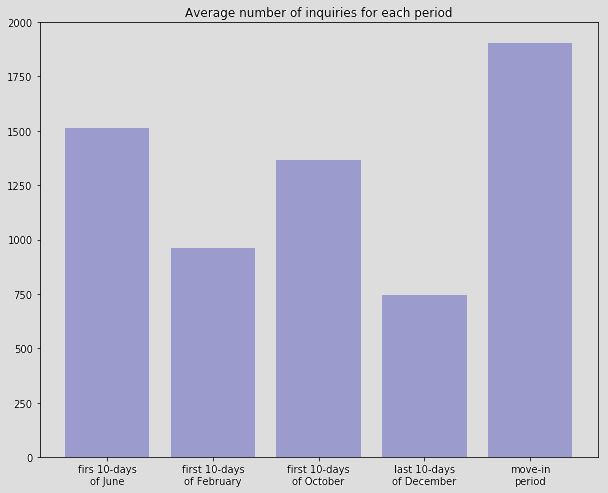
\includegraphics[width=\columnwidth]{inq.png}
\newline
\newline
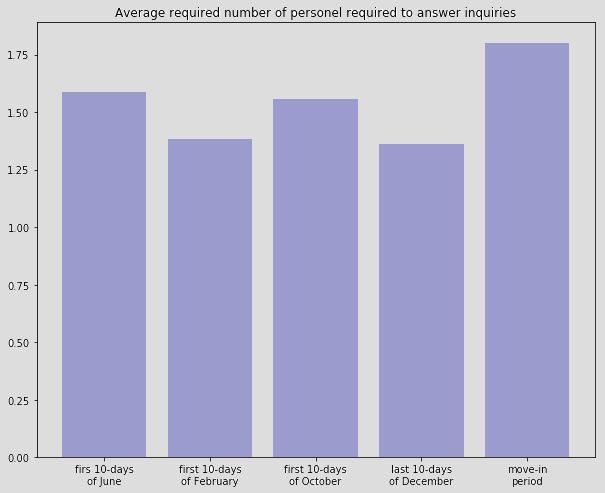
\includegraphics[width=\columnwidth]{pers.png}
% insert vincent's images
\newline

From the results we can see that the number of service requests and minimum
number of service request dispatchers is the highest during the move in period. To
be exact, number of inquiries is $47\%$ higher than the mean and minimum number of
dispatchers is $17\%$ higher than the mean during the move in period. If we assume
that the number of service requests and minimum number of dispatchers is
normally distributed and the mean and standard deviation in our results are
representative of the true distribution, the probability of having this high or a higher
result is $7.0\%$ for number of inquiries and $4.9\%$ for the minimum number of service
providers.

\subsection{Fire Incidents}
Reported fire incidents includes everything from smoke detector activations to electrical fires to cooking fires. Fire incidents negatively impact the wellbeing of the population of Boston, by damaging property, occupying safety services such as the Boston Fire Department, and impose a range to the general public. Our initial suspicion was that during move-in week, and during the time that colleges are in session, the fire department would be called more frequently and incident numbers would be higher. 

The fire incident datasets list the time, date, street address and the type of incident reported.  To better understand where most fire incidents occur, we decided to do a K-means clustering on the geolocations of fire incidents. To do this, we first used Google’s Geocoder API to transform the street addresses into geolocations, and then divided into three groups by month: May, September, and December. Then, K\-means clustering was applied to each of the periods. The K-means algorithm is initialized with k=2 (i.e 2 clusters) for each month, based on the K-means silhouette score being the highest for k=2 and significantly dropping for higher values of k. A high silhouette score indicates that each point has high similarity to its own cluster compared to other clusters. On the map below, you can see the resulting centroids from K\-means algorithm where red marks correspond to September, blue marks to May, and green marks to December.
\newline

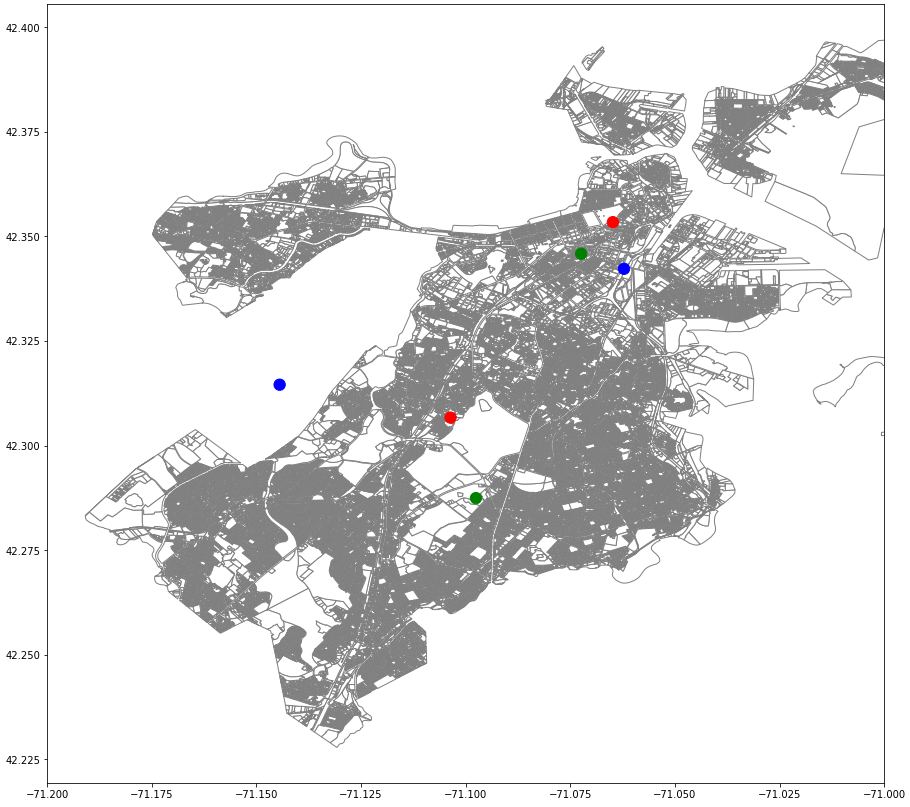
\includegraphics[width=\columnwidth]{fireMap.png}
\newline

Unfortunately, this map provides limited information because the two clusters seem to split the map into equal parts from the Southwest corner to the Northeast corner. The centroids seem to be covering as much of the geographical area as possible, leading us to believe that the fire incidents are almost uniformly distributed across Boston. This doesn’t lend itself to our initial hypothesis that the centroids would be closer to campuses and areas largely populated by students. That said, there is room for error in our results as about 15\% of the fire incidents were only listed by street name and not a specific number address.
\newline

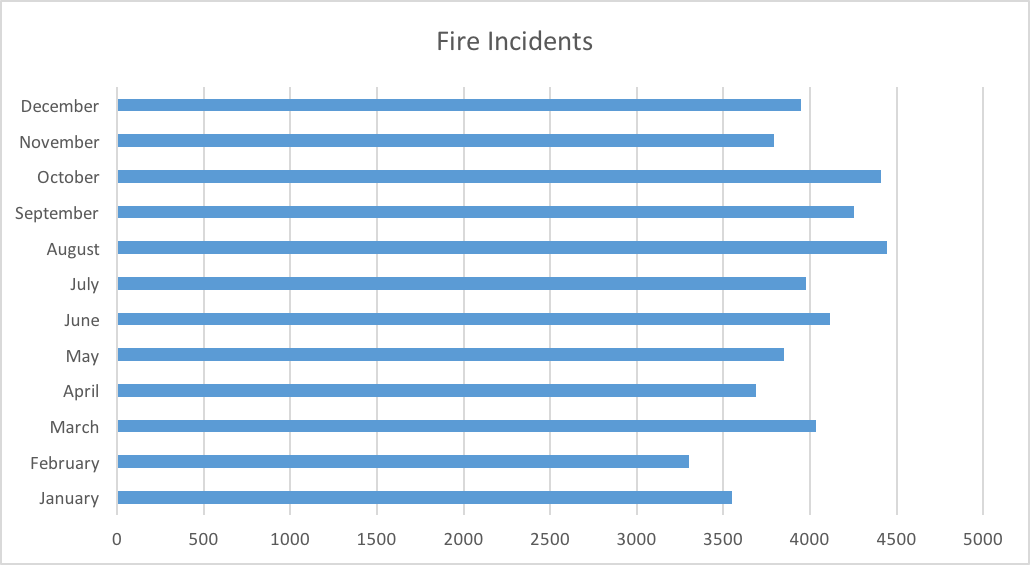
\includegraphics[width=\columnwidth]{fireChart.png}
\newline

This chart depicts the number of fire incidents for the first two weeks of each month. As you can see, the number of incidents is relatively consistent with August, March, and September reporting the highest numbers. 
We must account for the fact that move-in means the population of Boston increases, and thus the amount of incidents is likely to increase. That said, during other months with colleges in session, such as October and November, there are not as many incidents as in August and September.
The average number of fire incidents for all the months is $3,947.25$ incidents. For the months of August and September the average is $4,351.5$ fire incidents. This shows an increase of approximately 10\% for the move-in months. The standard deviation between the months is approximately $325.44$ incidents. Assuming number of incidents is normally distributed and the number of incidents is independent of the month, the probability of $4,351.5$ or more incidents in one month, is 11\%.
\subsection{Library Attendance Analysis}

\ Boston uses the CityScore initiative to measure the overall health of the city each day. The initiative aggregates various city metrics, both negative and additive, into a singular score. One of these metrics is public library users. The initiative’s goal is for this metric to increase, concluding with a higher score. To contest the notion that students decrease the quality of life in Boston, we examined how student library users impact the score in a positive way.
\newline

Our approach started with first filtering the CityScore dataset for entries that had the feature  [‘CTY\_SCR\_NAME’]  equal to ‘LIBRARY USERS’ [5]. Due to the student population in Boston, we hypothesized that the score would increase during the academic year. We divided our data based on the average academic calendar dates of Boston University, Northeastern University, Suffolk University, and the University of Massachusetts Boston. The dataset was projected into two different datasets:
\newline
\newline 
\textbf{LibraryNoStu:}
\newline
CityScore dates that fall into the part of the calendar year where students aren’t in session \newline[June, July, August, December 16th-31st, January 1st-15th]
\newline 
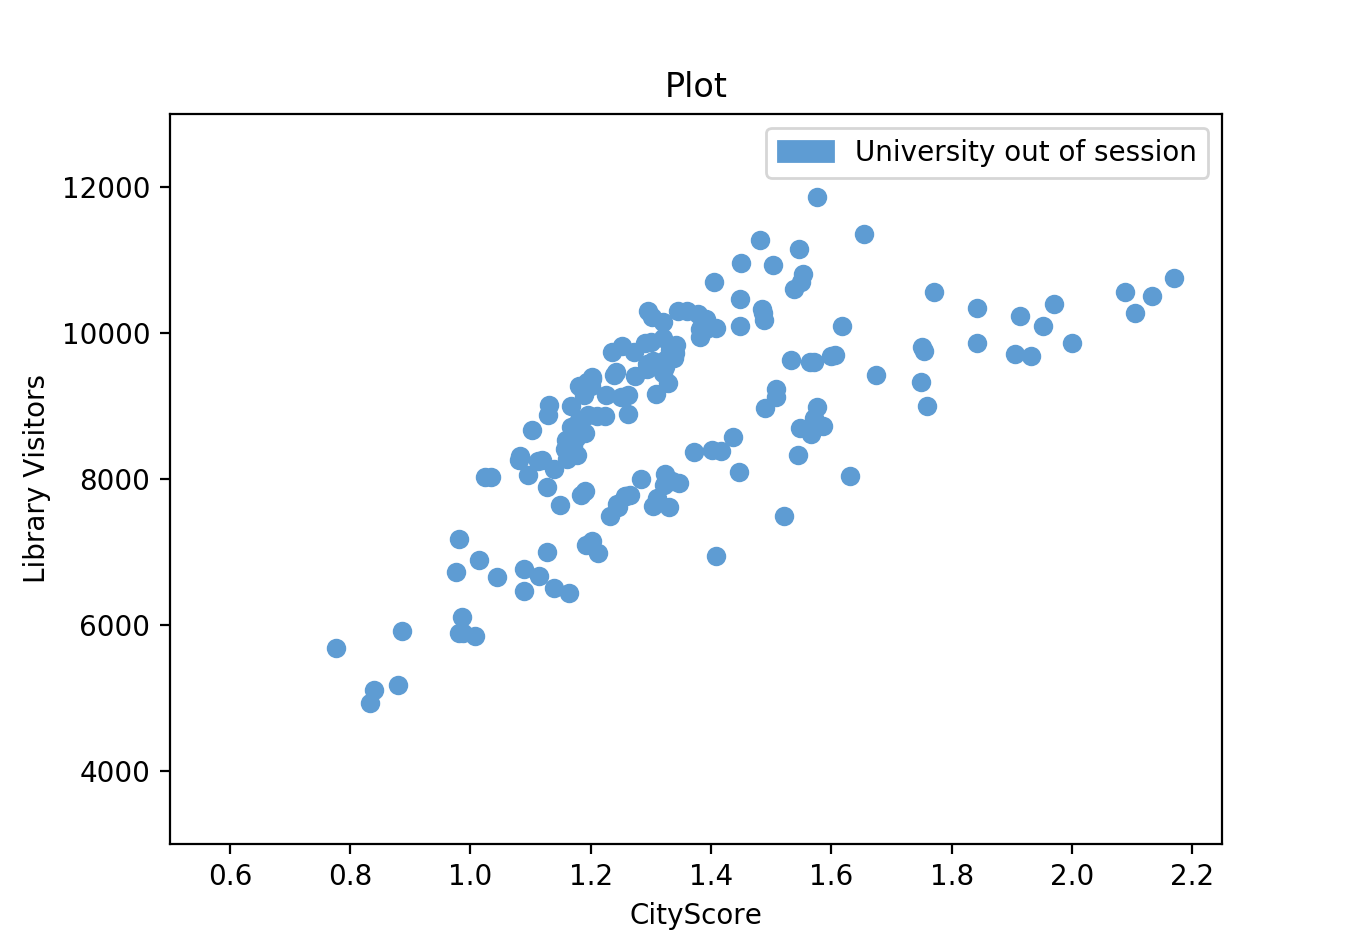
\includegraphics[width=\columnwidth]{noUniv.png}
\newline
\textbf{LibraryStu:}
\newline
CityScore dates that fall into the academic calendar of our control universities. \newline [September, October, November, December 1st-15th, January 16th-31st, February, March, April, May]
\newline 
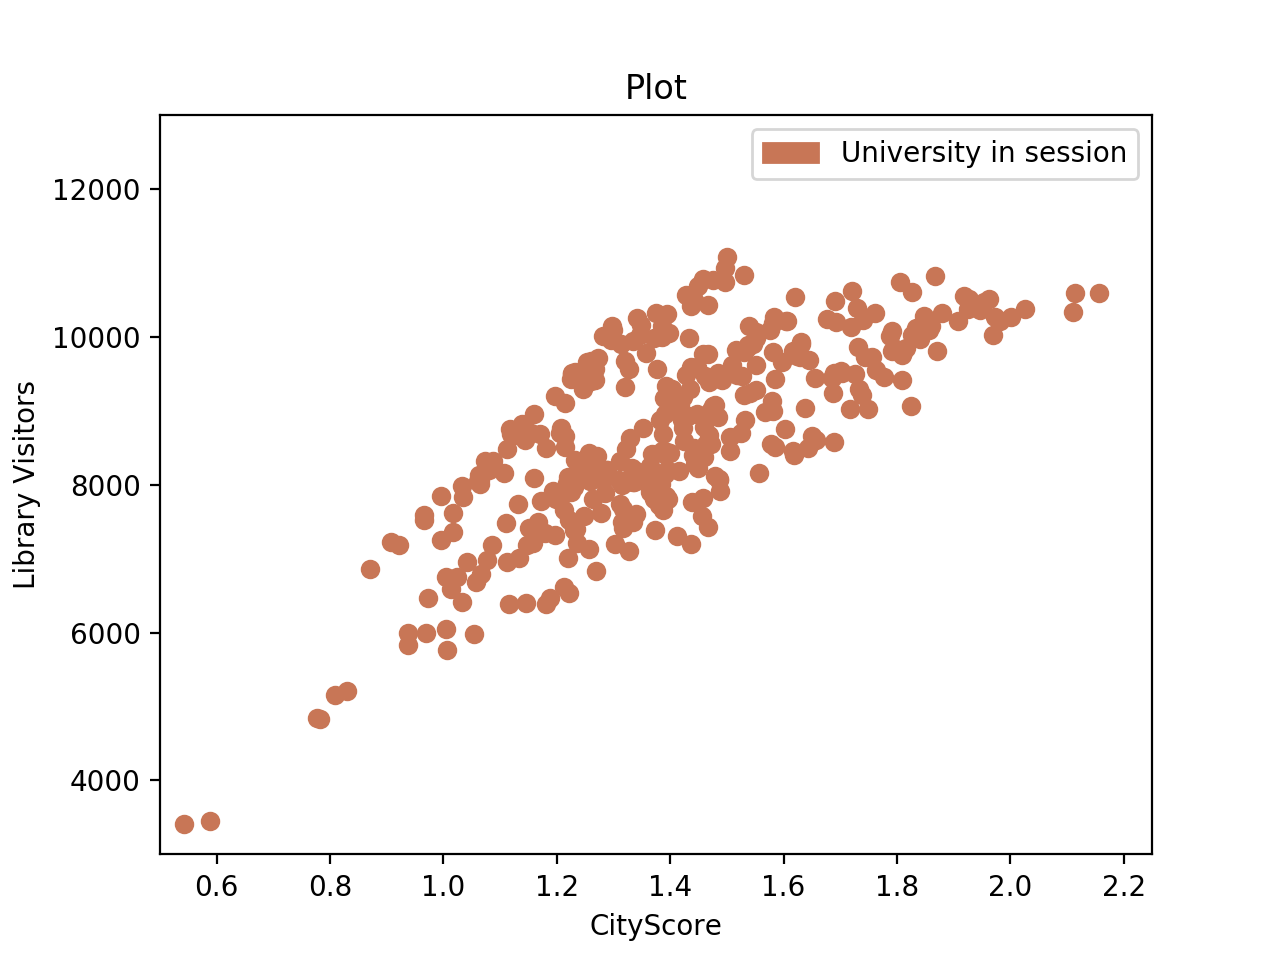
\includegraphics[width=\columnwidth]{Univ.png}
\newline 
\newline 
The trend of the scatter plot for each dataset showed a similar shape for both datasets. We calculated a correlation coefficient to examine the true correlation \cite{brookegh}.
\newline

$$\rho(x,y) = \frac{cov(x,y)}{(\sigma(x) * \sigma (y))}$$
where
$$\sigma = \ standard \  deviation\ = $$  
$$\sqrt{(\frac{1}{n})*((x_{1} - \mu(x))^{2}+...+(x_{n} - \mu(x))^{2}}$$
and
$$cov(x,y) = ((\frac{1}{\sqrt{(n)}})*(x-x_{\mu})) * ((\frac{1}{\sqrt{(n)}})) * (y-y_{mu}))$$
\newline
During the time that students are not in session, the correlation coefficient is .36, while during session it is .75. The result is that there is a stronger correlation between library users and CityScore during the academic year. In order for the city to achieve a higher daily CityScore, they should promote student library attendance.
\newline

While the correlation coefficient is higher during the academic calendar, something to keep in mind is that there is less data for attendance. In terms of average library visits, during the academic year there are 8721 visits on average and not during it there are 8845. So the average number of visits are actually higher during the time where there are less students.

\subsection{Analyzing Quality of Life}
Traditional economic indicators such as gross domestic product (GDP), Gini coefficient, and human development index (HDI) provide remarkable approximations for quality of life and are often indicative of a region's well-being and health \cite{gallup}\cite{wellbgallup}. In our analysis of Boston's quality of life, however, we avoid using these metrics for several reasons. First, the length of our timeframe of interest (7 days) renders the evolution of most economic indicators inconsequential. Second, given the geographic area of consideration (Greater Boston), none of the aforementioned metrics are appropriate\footnote{GDP, HDI, and Gini coefficients are computed for countries as a whole and are thus unlikely to register meaningful changes sparked by move-in week in one city.}. Perhaps most importantly, economic prosperity does not necessarily provide an accurate representation of emotional well-being \cite{wellbgallup}. 
\\In contrast, Twitter provides a rich source of data which, when analyzed, can reveal societal-scale levels of happiness \cite{happytexttwitter}. Twitter's erstwhile 140-character limit yields an extemporaneous dataset of user experiences \cite{moralsc}, especially given most Twitter users' proclivity for posting in the moment \cite{twtrends}\cite{mtwtrends}.
\\Dodds et al are careful to draw a distinction between experential/fleeting happiness and contentment and stress that their 'hedonometer' algorithm efficiently estimates the former, while inferring the latter with increasing accuracy over large periods of time \cite{happytext}.
\\Comparing multiple text corpora using a single metric necessitates justifying the variation. A comprehensive explanation of the 'word shift' graphs is provided in \cite{happytext}. We reproduce some of the calculations here:
\\Consider two texts $T_{ref}$ (for reference) and $T_{comp}$ (for comparison) with happiness scores $h_{avg}^{(ref)}$ and $h_{avg}^{(comp)}$, where the happiness score for a text is defined by:
\[h_{avg}(T) = \frac{\sum_{i=1}^{N}h_{avg}(w_{i})f_{i}}{\sum_{i=1}^{N}f_{i}} = \sum_{i=1}^{N}h_{avg}(w_i)p_i \quad\quad (1)\] where $f_i$ is the frequency of the $i^{th}$ word $w_i$ for which we have an estimate of average happiness, $h_{avg}(w_i)$, and $p_i = \frac{f_i}{\sum_{j=1}^{N}f_j}$ represents the corresponding normalized frequency\footnote{The average happiness for over 10,000 words was calculated and made publicly available as part of the labMT dataset by Dodds et al}.
\\Using Eq (1), we can compare two texts thus:
\[h_{avg}^{(comp)} - h_{avg}^{(ref)} = \sum_{i=1}^{N}h_{avg}(w_i)[p_i^{(comp)} - p_i^{(ref)}]\]
\[= \sum_{i=1}^{N}[h_{avg}(w_i) - h_{avg}^{(ref)}][p_i^{(comp)} - p_i^{(ref)}] \quad (2)\]
\[\because \sum_{i=1}^{N}h_{avg}^{(ref)}[p_i^{(comp)} - p_i^{(ref)}] = h_{avg}^{(ref)}[p_i^{(comp)} - p_i^{(ref)}]\]
\[= h_{avg}^{(ref)}(1-1) = 0\]
Two aspects determine the change in the $i^{th}$ word's contribution:
\\\null\quad\quad1. Whether the word is (on average) happier than the reference text's average, $h_{avg}^{(ref)}$ and
\\\null\quad\quad2. The relative abundance of the word in $T_{comp}$ to that in $T_{ref}$.
\\A word's happiness relative to $T_{ref}$ is specified by $+$ (happier) and $-$ (less happier).
\\Relative abundance is specified similarly, using $\uparrow$ (more abundant) and $\downarrow$ (less abundant).
\\The combination of both results in the following four possibilities:
\\\null\quad\quad1. $+\uparrow:$ Increased usage of relatively positive words.
\\\null\quad\quad2. $-\downarrow:$ Decreased usage of relatively negative words.
\\\null\quad\quad3. $+\downarrow:$ Decreased usage of relatively positive words.
\\\null\quad\quad4. $-\uparrow:$ Increased usage of relatively negative words.
\\Eq (2) is normalized to obtain a normalized summand:
\[\delta h_{avg,i} = \frac{100}{|h_{avg}^{(comp)} - h_{avg}^{(ref)}]} t\]
where \[t = \underbrace{[h_{avg}(w_i) - h_{avg}^{(ref)}]}_{+/-} \underbrace{[p_{i}^{(comp)} - p_{i}^{(ref)}]}_{\uparrow/\downarrow} \quad(3)\]
where $\sum_{i}\delta h_{avg,i} = \pm100$
\\\\A demonstration of this is provided in figure \ref{fig:wordshift0}, using the \textit{dharmSentiment} module \cite{dharmsentiment}.
    \begin{figure}[!hbt]
        \begin{center}
        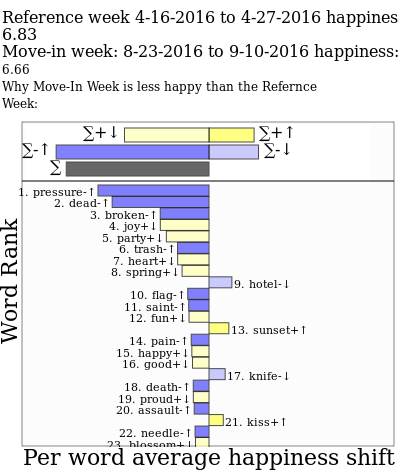
\includegraphics[width=\columnwidth]{wordshift0}
        \caption{A comparison of the happiness between move-in week and a randomly chosen week during the summer.}
        \label{fig:wordshift0}
        \end{center}
    \end{figure}
    Clearly, the negative words pressure, dead, broken, and trash were used more frequently, while the positive words joy, party, heart, and spring were used less frequently. 

\section{Conclusion}
Our perfunctory investigation of the relationship between move-in week and quality of life is indicative of a negative correlation between move-in week and quality of life. While happiness (which was a heavily weighted component in our estimations of quality of life) is admittedly subjective and self-reported, we are confident that our approach to its evaluation provides a tenable, if somewhat inscrutable picture of happiness for the population as a whole. Time and primarily computational constraints prevented us from developing an inferential model of the shift in public happiness, given some of the optimizations suggested in section III, but we are hopeful that future work will explore this.
\\The work done in this paper would not have been possible without the 'hedonometer algorithm', or the \textit{simpleLabMT} software package \cite{simplelabmt},  both of which were designed in part by Dr. Andrew Reagan at the University of Vermont.

% Now we need a bibliography:
\begin{thebibliography}{5}

    %Each item starts with a \bibitem{reference} command and the details thereafter.
    \bibitem{painfulmovein}
    Landry, Lauren. "Boston, You've Been Warned: The College Students Are Here.? Americaninno.com, 25 Aug. 2014, www.americaninno.com/boston/move-in-dates-for-boston-college-students-back-to-school-in-boston/.
    
    \bibitem{moveinstats}
    United States, Congress, Meade, Peter. "Boston by the Numbers: Colleges and Universities" Boston Redevelopment Authority. www.bostonplans.org/getattachment/1770c181-7878-47ab-892f-84baca828bf3 2011.
    
    \bibitem{storrowed}
    Slane, Kevin. "Trillium Has a New Beer Named for Trucks That Get 'Storrowed'." Boston.com, The Boston Globe, 2 Feb. 2018, https://www.boston.com/culture/lifestyle/2018/02/02/trillium-has-a-new-beer-named-for-trucks-that-get-storrowed.
    
    \bibitem{happytext}
    Dodds, Peter Sheridan, et al. "Temporal patterns of happiness and information in a global social network: Hedonometrics and Twitter." PloS one 6.12 (2011): e26752.
    
    \bibitem{bosdatalink}
    Analyze Boston, https://data.boston.gov/.

   \bibitem{twitterlink}
   Twitter, https://twitter.com.
   
   \bibitem{trashcity}
   J.~Haddidin,  \emph{Trash City: How Does Moving Week Impact the Quality of Life in Boston?},\relax Analyze Boston,  \emph{https://data.boston.gov/showcase/trash-city}
   
   \bibitem{happytexttwitter}
   Mitchell, Lewis, et al. "The geography of happiness: Connecting twitter sentiment and expression, demographics, and objective characteristics of place." PloS one 8.5 (2013): e64417.
   
   \bibitem{gallup}
   Diener, Ed. "Subjective well-being: The science of happiness and a proposal for a national index." American psychologist 55.1 (2000): 34.
   
   \bibitem{simplelabmt}
   andyreagan/labMT-simple
"Andyreagan/Labmt-Simple." GitHub. N. p., 2018. Web. 30 Apr. 2018.
   
   \bibitem{wellbgallup}
   Kahneman, Daniel, and Angus Deaton. "High income improves evaluation of life but not emotional well-being." Proceedings of the national academy of sciences 107.38 (2010): 16489-16493.
   
   \bibitem{moralsc}
   Edgeworth, Francis Ysidro. Mathematical psychics: An essay on the application of mathematics to the moral sciences. Vol. 10. Kegan Paul, 1881.
   
   \bibitem{twtrends}
   Dunlap, Joanna C., and Patrick R. Lowenthal. "Tweeting the night away: Using Twitter to enhance social presence." Journal of Information Systems Education 20.2 (2009): 129.
   
   \bibitem{dharmsentiment}
   Tarapore, Dharmesh. "Weirdindiankid/Dharmsentiment." GitHub. 2018. Web. 30 Apr. 2018, URL https://github.com/weirdindiankid/dharmSentiment
   
   \bibitem{mtwtrends}
   Bruns, Axel, and Jean E. Burgess. "The use of Twitter hashtags in the formation of ad hoc publics." Proceedings of the 6th European Consortium for Political Research (ECPR) General Conference 2011. 2011.
   
   \bibitem{tlim}
   Inside Twitter: An In-Depth Look Inside the Twitter World, Sysmos Resource Library. Available at http:// www.sysomos.com/insidetwitter/. Accessed April 12, 2018.
   
   \bibitem{tlim2}
   S. Fox, K. Zickuhr, and A. Smith, Tech. Rep., Pew Internet \& American Life Project (2006), accessed April 13, 2018, URL http://www.pewinternet.org/Reports/
2009/17-Twitter-and-Status-Updating-Fall-2009.
aspx.
   
   \bibitem{tthpp}
   D. Kahneman and J. Riis, in The science of well-being,
edited by F. A. Huppert, N. Baylis, and B. Keverne
(Oxford University Press, Oxford, UK, 2005), pp. 285?
304
   
   \bibitem{thpp}
   M. A. Killingsworth and D. T. Gilbert, Science Magazine
   330, 932 (2010)
   
   \bibitem{brookegh}
   Mullen, Brooke "StatLib.py" GitHub. 2018. Web. 01 May. 2018, URL https://github.com/Data-Mechanics/course-2018-spr-proj/blob/master/bemullen\_crussack\_dharmesh\_vinwah/StatLibrary.py

\end{thebibliography}

% Your document ends here!
\end{document}